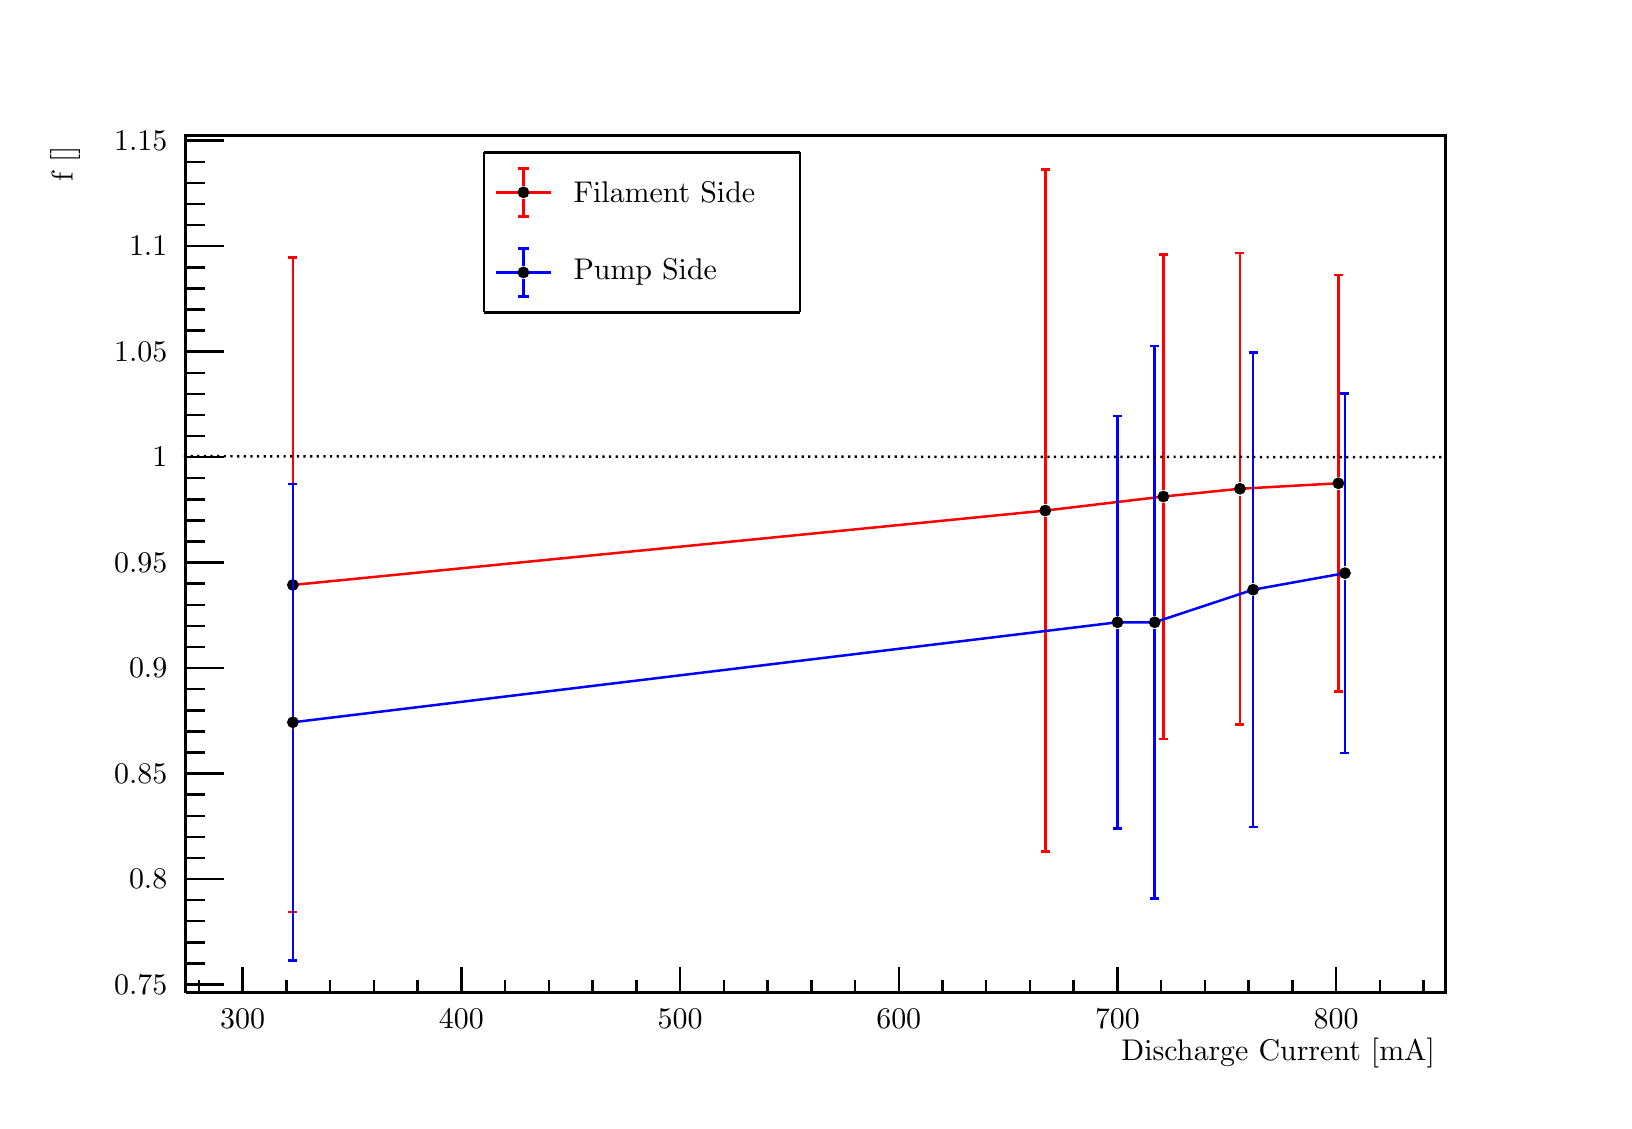
\begin{tikzpicture}
\pgfdeclareplotmark{cross} {
\pgfpathmoveto{\pgfpoint{-0.3\pgfplotmarksize}{\pgfplotmarksize}}
\pgfpathlineto{\pgfpoint{+0.3\pgfplotmarksize}{\pgfplotmarksize}}
\pgfpathlineto{\pgfpoint{+0.3\pgfplotmarksize}{0.3\pgfplotmarksize}}
\pgfpathlineto{\pgfpoint{+1\pgfplotmarksize}{0.3\pgfplotmarksize}}
\pgfpathlineto{\pgfpoint{+1\pgfplotmarksize}{-0.3\pgfplotmarksize}}
\pgfpathlineto{\pgfpoint{+0.3\pgfplotmarksize}{-0.3\pgfplotmarksize}}
\pgfpathlineto{\pgfpoint{+0.3\pgfplotmarksize}{-1.\pgfplotmarksize}}
\pgfpathlineto{\pgfpoint{-0.3\pgfplotmarksize}{-1.\pgfplotmarksize}}
\pgfpathlineto{\pgfpoint{-0.3\pgfplotmarksize}{-0.3\pgfplotmarksize}}
\pgfpathlineto{\pgfpoint{-1.\pgfplotmarksize}{-0.3\pgfplotmarksize}}
\pgfpathlineto{\pgfpoint{-1.\pgfplotmarksize}{0.3\pgfplotmarksize}}
\pgfpathlineto{\pgfpoint{-0.3\pgfplotmarksize}{0.3\pgfplotmarksize}}
\pgfpathclose
\pgfusepathqstroke
}
\pgfdeclareplotmark{cross*} {
\pgfpathmoveto{\pgfpoint{-0.3\pgfplotmarksize}{\pgfplotmarksize}}
\pgfpathlineto{\pgfpoint{+0.3\pgfplotmarksize}{\pgfplotmarksize}}
\pgfpathlineto{\pgfpoint{+0.3\pgfplotmarksize}{0.3\pgfplotmarksize}}
\pgfpathlineto{\pgfpoint{+1\pgfplotmarksize}{0.3\pgfplotmarksize}}
\pgfpathlineto{\pgfpoint{+1\pgfplotmarksize}{-0.3\pgfplotmarksize}}
\pgfpathlineto{\pgfpoint{+0.3\pgfplotmarksize}{-0.3\pgfplotmarksize}}
\pgfpathlineto{\pgfpoint{+0.3\pgfplotmarksize}{-1.\pgfplotmarksize}}
\pgfpathlineto{\pgfpoint{-0.3\pgfplotmarksize}{-1.\pgfplotmarksize}}
\pgfpathlineto{\pgfpoint{-0.3\pgfplotmarksize}{-0.3\pgfplotmarksize}}
\pgfpathlineto{\pgfpoint{-1.\pgfplotmarksize}{-0.3\pgfplotmarksize}}
\pgfpathlineto{\pgfpoint{-1.\pgfplotmarksize}{0.3\pgfplotmarksize}}
\pgfpathlineto{\pgfpoint{-0.3\pgfplotmarksize}{0.3\pgfplotmarksize}}
\pgfpathclose
\pgfusepathqfillstroke
}
\pgfdeclareplotmark{newstar} {
\pgfpathmoveto{\pgfqpoint{0pt}{\pgfplotmarksize}}
\pgfpathlineto{\pgfqpointpolar{44}{0.5\pgfplotmarksize}}
\pgfpathlineto{\pgfqpointpolar{18}{\pgfplotmarksize}}
\pgfpathlineto{\pgfqpointpolar{-20}{0.5\pgfplotmarksize}}
\pgfpathlineto{\pgfqpointpolar{-54}{\pgfplotmarksize}}
\pgfpathlineto{\pgfqpointpolar{-90}{0.5\pgfplotmarksize}}
\pgfpathlineto{\pgfqpointpolar{234}{\pgfplotmarksize}}
\pgfpathlineto{\pgfqpointpolar{198}{0.5\pgfplotmarksize}}
\pgfpathlineto{\pgfqpointpolar{162}{\pgfplotmarksize}}
\pgfpathlineto{\pgfqpointpolar{134}{0.5\pgfplotmarksize}}
\pgfpathclose
\pgfusepathqstroke
}
\pgfdeclareplotmark{newstar*} {
\pgfpathmoveto{\pgfqpoint{0pt}{\pgfplotmarksize}}
\pgfpathlineto{\pgfqpointpolar{44}{0.5\pgfplotmarksize}}
\pgfpathlineto{\pgfqpointpolar{18}{\pgfplotmarksize}}
\pgfpathlineto{\pgfqpointpolar{-20}{0.5\pgfplotmarksize}}
\pgfpathlineto{\pgfqpointpolar{-54}{\pgfplotmarksize}}
\pgfpathlineto{\pgfqpointpolar{-90}{0.5\pgfplotmarksize}}
\pgfpathlineto{\pgfqpointpolar{234}{\pgfplotmarksize}}
\pgfpathlineto{\pgfqpointpolar{198}{0.5\pgfplotmarksize}}
\pgfpathlineto{\pgfqpointpolar{162}{\pgfplotmarksize}}
\pgfpathlineto{\pgfqpointpolar{134}{0.5\pgfplotmarksize}}
\pgfpathclose
\pgfusepathqfillstroke
}
\definecolor{c}{rgb}{1,1,1};
\draw [color=c, fill=c] (0,0) rectangle (20,13.6103);
\draw [color=c, fill=c] (2,1.36103) rectangle (18,12.2493);
\definecolor{c}{rgb}{0,0,0};
\draw [c,line width=0.9] (2,1.36103) -- (2,12.2493) -- (18,12.2493) -- (18,1.36103) -- (2,1.36103);
\definecolor{c}{rgb}{1,1,1};
\draw [color=c, fill=c] (2,1.36103) rectangle (18,12.2493);
\definecolor{c}{rgb}{0,0,0};
\draw [c,line width=0.9] (2,1.36103) -- (2,12.2493) -- (18,12.2493) -- (18,1.36103) -- (2,1.36103);
\draw [c,line width=0.9] (2,1.36103) -- (18,1.36103);
\draw [c,line width=0.9] (2.72222,1.68768) -- (2.72222,1.36103);
\draw [c,line width=0.9] (3.27778,1.52436) -- (3.27778,1.36103);
\draw [c,line width=0.9] (3.83333,1.52436) -- (3.83333,1.36103);
\draw [c,line width=0.9] (4.38889,1.52436) -- (4.38889,1.36103);
\draw [c,line width=0.9] (4.94444,1.52436) -- (4.94444,1.36103);
\draw [c,line width=0.9] (5.5,1.68768) -- (5.5,1.36103);
\draw [c,line width=0.9] (6.05556,1.52436) -- (6.05556,1.36103);
\draw [c,line width=0.9] (6.61111,1.52436) -- (6.61111,1.36103);
\draw [c,line width=0.9] (7.16667,1.52436) -- (7.16667,1.36103);
\draw [c,line width=0.9] (7.72222,1.52436) -- (7.72222,1.36103);
\draw [c,line width=0.9] (8.27778,1.68768) -- (8.27778,1.36103);
\draw [c,line width=0.9] (8.83333,1.52436) -- (8.83333,1.36103);
\draw [c,line width=0.9] (9.38889,1.52436) -- (9.38889,1.36103);
\draw [c,line width=0.9] (9.94444,1.52436) -- (9.94444,1.36103);
\draw [c,line width=0.9] (10.5,1.52436) -- (10.5,1.36103);
\draw [c,line width=0.9] (11.0556,1.68768) -- (11.0556,1.36103);
\draw [c,line width=0.9] (11.6111,1.52436) -- (11.6111,1.36103);
\draw [c,line width=0.9] (12.1667,1.52436) -- (12.1667,1.36103);
\draw [c,line width=0.9] (12.7222,1.52436) -- (12.7222,1.36103);
\draw [c,line width=0.9] (13.2778,1.52436) -- (13.2778,1.36103);
\draw [c,line width=0.9] (13.8333,1.68768) -- (13.8333,1.36103);
\draw [c,line width=0.9] (14.3889,1.52436) -- (14.3889,1.36103);
\draw [c,line width=0.9] (14.9444,1.52436) -- (14.9444,1.36103);
\draw [c,line width=0.9] (15.5,1.52436) -- (15.5,1.36103);
\draw [c,line width=0.9] (16.0556,1.52436) -- (16.0556,1.36103);
\draw [c,line width=0.9] (16.6111,1.68768) -- (16.6111,1.36103);
\draw [c,line width=0.9] (2.72222,1.68768) -- (2.72222,1.36103);
\draw [c,line width=0.9] (2.16667,1.52436) -- (2.16667,1.36103);
\draw [c,line width=0.9] (16.6111,1.68768) -- (16.6111,1.36103);
\draw [c,line width=0.9] (17.1667,1.52436) -- (17.1667,1.36103);
\draw [c,line width=0.9] (17.7222,1.52436) -- (17.7222,1.36103);
\draw [anchor=base] (2.72222,0.911891) node[scale=1.08185, color=c, rotate=0]{300};
\draw [anchor=base] (5.5,0.911891) node[scale=1.08185, color=c, rotate=0]{400};
\draw [anchor=base] (8.27778,0.911891) node[scale=1.08185, color=c, rotate=0]{500};
\draw [anchor=base] (11.0556,0.911891) node[scale=1.08185, color=c, rotate=0]{600};
\draw [anchor=base] (13.8333,0.911891) node[scale=1.08185, color=c, rotate=0]{700};
\draw [anchor=base] (16.6111,0.911891) node[scale=1.08185, color=c, rotate=0]{800};
\draw [anchor= east] (18,0.598854) node[scale=1.08185, color=c, rotate=0]{Discharge Current [mA]};
\draw [c,line width=0.9] (2,1.36103) -- (2,12.2493);
\draw [c,line width=0.9] (2.48,1.46562) -- (2,1.46562);
\draw [c,line width=0.9] (2.24,1.73351) -- (2,1.73351);
\draw [c,line width=0.9] (2.24,2.00141) -- (2,2.00141);
\draw [c,line width=0.9] (2.24,2.2693) -- (2,2.2693);
\draw [c,line width=0.9] (2.24,2.5372) -- (2,2.5372);
\draw [c,line width=0.9] (2.48,2.80509) -- (2,2.80509);
\draw [c,line width=0.9] (2.24,3.07299) -- (2,3.07299);
\draw [c,line width=0.9] (2.24,3.34088) -- (2,3.34088);
\draw [c,line width=0.9] (2.24,3.60878) -- (2,3.60878);
\draw [c,line width=0.9] (2.24,3.87667) -- (2,3.87667);
\draw [c,line width=0.9] (2.48,4.14456) -- (2,4.14456);
\draw [c,line width=0.9] (2.24,4.41246) -- (2,4.41246);
\draw [c,line width=0.9] (2.24,4.68035) -- (2,4.68035);
\draw [c,line width=0.9] (2.24,4.94825) -- (2,4.94825);
\draw [c,line width=0.9] (2.24,5.21614) -- (2,5.21614);
\draw [c,line width=0.9] (2.48,5.48404) -- (2,5.48404);
\draw [c,line width=0.9] (2.24,5.75193) -- (2,5.75193);
\draw [c,line width=0.9] (2.24,6.01982) -- (2,6.01982);
\draw [c,line width=0.9] (2.24,6.28772) -- (2,6.28772);
\draw [c,line width=0.9] (2.24,6.55561) -- (2,6.55561);
\draw [c,line width=0.9] (2.48,6.82351) -- (2,6.82351);
\draw [c,line width=0.9] (2.24,7.0914) -- (2,7.0914);
\draw [c,line width=0.9] (2.24,7.3593) -- (2,7.3593);
\draw [c,line width=0.9] (2.24,7.62719) -- (2,7.62719);
\draw [c,line width=0.9] (2.24,7.89509) -- (2,7.89509);
\draw [c,line width=0.9] (2.48,8.16298) -- (2,8.16298);
\draw [c,line width=0.9] (2.24,8.43087) -- (2,8.43087);
\draw [c,line width=0.9] (2.24,8.69877) -- (2,8.69877);
\draw [c,line width=0.9] (2.24,8.96666) -- (2,8.96666);
\draw [c,line width=0.9] (2.24,9.23456) -- (2,9.23456);
\draw [c,line width=0.9] (2.48,9.50245) -- (2,9.50245);
\draw [c,line width=0.9] (2.24,9.77035) -- (2,9.77035);
\draw [c,line width=0.9] (2.24,10.0382) -- (2,10.0382);
\draw [c,line width=0.9] (2.24,10.3061) -- (2,10.3061);
\draw [c,line width=0.9] (2.24,10.574) -- (2,10.574);
\draw [c,line width=0.9] (2.48,10.8419) -- (2,10.8419);
\draw [c,line width=0.9] (2.24,11.1098) -- (2,11.1098);
\draw [c,line width=0.9] (2.24,11.3777) -- (2,11.3777);
\draw [c,line width=0.9] (2.24,11.6456) -- (2,11.6456);
\draw [c,line width=0.9] (2.24,11.9135) -- (2,11.9135);
\draw [c,line width=0.9] (2.48,12.1814) -- (2,12.1814);
\draw [c,line width=0.9] (2.48,1.46562) -- (2,1.46562);
\draw [c,line width=0.9] (2.48,12.1814) -- (2,12.1814);
\draw [anchor= east] (1.9,1.46562) node[scale=1.08185, color=c, rotate=0]{0.75};
\draw [anchor= east] (1.9,2.80509) node[scale=1.08185, color=c, rotate=0]{0.8};
\draw [anchor= east] (1.9,4.14456) node[scale=1.08185, color=c, rotate=0]{0.85};
\draw [anchor= east] (1.9,5.48404) node[scale=1.08185, color=c, rotate=0]{0.9};
\draw [anchor= east] (1.9,6.82351) node[scale=1.08185, color=c, rotate=0]{0.95};
\draw [anchor= east] (1.9,8.16298) node[scale=1.08185, color=c, rotate=0]{1};
\draw [anchor= east] (1.9,9.50245) node[scale=1.08185, color=c, rotate=0]{1.05};
\draw [anchor= east] (1.9,10.8419) node[scale=1.08185, color=c, rotate=0]{1.1};
\draw [anchor= east] (1.9,12.1814) node[scale=1.08185, color=c, rotate=0]{1.15};
\draw [anchor= east] (0.469055,12.2493) node[scale=1.08185, color=c, rotate=90]{f []};
\definecolor{c}{rgb}{1,0,0};
\draw [c,line width=0.9] (3.36111,6.53969) -- (12.9167,7.48458) -- (14.4167,7.66271) -- (15.3889,7.76169) -- (16.6389,7.83092);
\definecolor{c}{rgb}{0,0,0};
\foreach \P in {(3.36111,6.53969), (12.9167,7.48458), (14.4167,7.66271), (15.3889,7.76169), (16.6389,7.83092)}{\draw[mark options={color=c,fill=c},mark size=1.921922pt,mark=*] plot coordinates {\P};}
\definecolor{c}{rgb}{1,0,0};
\draw [c,line width=0.9] (3.36111,6.62565) -- (3.36111,10.6954);
\draw [c,line width=0.9] (3.3038,10.6954) -- (3.41842,10.6954);
\draw [c,line width=0.9] (3.36111,6.45373) -- (3.36111,2.38397);
\draw [c,line width=0.9] (3.3038,2.38397) -- (3.41842,2.38397);
\draw [c,line width=0.9] (12.9167,7.57054) -- (12.9167,11.817);
\draw [c,line width=0.9] (12.8594,11.817) -- (12.974,11.817);
\draw [c,line width=0.9] (12.9167,7.39862) -- (12.9167,3.15219);
\draw [c,line width=0.9] (12.8594,3.15219) -- (12.974,3.15219);
\draw [c,line width=0.9] (14.4167,7.74867) -- (14.4167,10.7388);
\draw [c,line width=0.9] (14.3594,10.7388) -- (14.474,10.7388);
\draw [c,line width=0.9] (14.4167,7.57675) -- (14.4167,4.58665);
\draw [c,line width=0.9] (14.3594,4.58665) -- (14.474,4.58665);
\draw [c,line width=0.9] (15.3889,7.84765) -- (15.3889,10.7537);
\draw [c,line width=0.9] (15.3316,10.7537) -- (15.4462,10.7537);
\draw [c,line width=0.9] (15.3889,7.67573) -- (15.3889,4.76969);
\draw [c,line width=0.9] (15.3316,4.76969) -- (15.4462,4.76969);
\draw [c,line width=0.9] (16.6389,7.91688) -- (16.6389,10.4756);
\draw [c,line width=0.9] (16.5816,10.4756) -- (16.6962,10.4756);
\draw [c,line width=0.9] (16.6389,7.74496) -- (16.6389,5.1862);
\draw [c,line width=0.9] (16.5816,5.1862) -- (16.6962,5.1862);
\definecolor{c}{rgb}{0,0,1};
\draw [c,line width=0.9] (3.36111,4.88167) -- (3.36111,7.82117);
\draw [c,line width=0.9] (3.3038,7.82117) -- (3.41842,7.82117);
\draw [c,line width=0.9] (3.36111,4.70975) -- (3.36111,1.77026);
\draw [c,line width=0.9] (3.3038,1.77026) -- (3.41842,1.77026);
\draw [c,line width=0.9] (13.8333,6.15176) -- (13.8333,8.6827);
\draw [c,line width=0.9] (13.776,8.6827) -- (13.8906,8.6827);
\draw [c,line width=0.9] (13.8333,5.97984) -- (13.8333,3.4489);
\draw [c,line width=0.9] (13.776,3.4489) -- (13.8906,3.4489);
\draw [c,line width=0.9] (14.3056,6.15176) -- (14.3056,9.57385);
\draw [c,line width=0.9] (14.2482,9.57385) -- (14.3629,9.57385);
\draw [c,line width=0.9] (14.3056,5.97984) -- (14.3056,2.55775);
\draw [c,line width=0.9] (14.2482,2.55775) -- (14.3629,2.55775);
\draw [c,line width=0.9] (15.5556,6.56543) -- (15.5556,9.491);
\draw [c,line width=0.9] (15.4982,9.491) -- (15.6129,9.491);
\draw [c,line width=0.9] (15.5556,6.39351) -- (15.5556,3.46793);
\draw [c,line width=0.9] (15.4982,3.46793) -- (15.6129,3.46793);
\draw [c,line width=0.9] (16.7222,6.7758) -- (16.7222,8.97269);
\draw [c,line width=0.9] (16.6649,8.97269) -- (16.7795,8.97269);
\draw [c,line width=0.9] (16.7222,6.60388) -- (16.7222,4.40699);
\draw [c,line width=0.9] (16.6649,4.40699) -- (16.7795,4.40699);
\draw [c,line width=0.9] (3.36111,4.79571) -- (13.8333,6.0658) -- (14.3056,6.0658) -- (15.5556,6.47947) -- (16.7222,6.68984);
\definecolor{c}{rgb}{0,0,0};
\foreach \P in {(3.36111,4.79571), (13.8333,6.0658), (14.3056,6.0658), (15.5556,6.47947), (16.7222,6.68984)}{\draw[mark options={color=c,fill=c},mark size=1.921922pt,mark=*] plot coordinates {\P};}
\definecolor{c}{rgb}{1,1,1};
\draw [color=c, fill=c] (5.78797,10) rectangle (9.79943,12.0344);
\definecolor{c}{rgb}{0,0,0};
\draw [c,line width=0.9] (5.78797,10) -- (9.79943,10);
\draw [c,line width=0.9] (9.79943,10) -- (9.79943,12.0344);
\draw [c,line width=0.9] (9.79943,12.0344) -- (5.78797,12.0344);
\draw [c,line width=0.9] (5.78797,12.0344) -- (5.78797,10);
\draw [anchor= west] (6.79083,11.5258) node[scale=1.08185, color=c, rotate=0]{Filament Side};
\definecolor{c}{rgb}{1,0,0};
\draw [c,line width=0.9] (5.9384,11.5258) -- (6.6404,11.5258);
\draw [c,line width=0.9] (6.2894,11.6117) -- (6.2894,11.8309);
\draw [c,line width=0.9] (6.2894,11.4398) -- (6.2894,11.2206);
\draw [c,line width=0.9] (6.2192,11.8309) -- (6.3596,11.8309);
\draw [c,line width=0.9] (6.2192,11.2206) -- (6.3596,11.2206);
\definecolor{c}{rgb}{0,0,0};
\foreach \P in {(6.2894,11.5258)}{\draw[mark options={color=c,fill=c},mark size=1.921922pt,mark=*] plot coordinates {\P};}
\draw [anchor= west] (6.79083,10.5086) node[scale=1.08185, color=c, rotate=0]{Pump Side};
\definecolor{c}{rgb}{0,0,1};
\draw [c,line width=0.9] (5.9384,10.5086) -- (6.6404,10.5086);
\draw [c,line width=0.9] (6.2894,10.5946) -- (6.2894,10.8138);
\draw [c,line width=0.9] (6.2894,10.4226) -- (6.2894,10.2034);
\draw [c,line width=0.9] (6.2192,10.8138) -- (6.3596,10.8138);
\draw [c,line width=0.9] (6.2192,10.2034) -- (6.3596,10.2034);
\definecolor{c}{rgb}{0,0,0};
\foreach \P in {(6.2894,10.5086)}{\draw[mark options={color=c,fill=c},mark size=1.921922pt,mark=*] plot coordinates {\P};}
\draw [c,dash pattern=on 0.80pt off 1.60pt ,line width=0.9] (1.97708,8.17475) -- (17.9943,8.16298);
\end{tikzpicture}
